\documentclass[12pt]{article}
\usepackage{light}
\hidesolutions
%\showsolutions

%%%%% some macros needed %%%%%%%%%%%
\newcommand{\eqdef}{\mathbin{::=}}
\newcommand{\mfigure}[3]{\bigskip\centerline{\resizebox{#1}{#2}{\includegraphics{#3}}}\bigskip}
\newcommand{\edge}[2]{#1\text{---}#2}
\newcommand{\arc}[2]{#1\!\longrightarrow\!#2}
\newcommand{\beqn}{\begin{eqnarray*}}
\newcommand{\eeqn}{\end{eqnarray*}}
\newcommand{\ok}{\marginpar{ok?}}
%%%%%%%%%%%%%%%%%%%%%%%%%%%%%%%%%%%%%

\begin{document}

\recitation{8}{\today}
\section{Build-up error}
Recall a graph is \term{connected} iff there is a path between every pair of its vertices.

\begin{falseclm*}
If every vertex in a graph has positive degree, then the graph is
connected.
\end{falseclm*}

\begin{enumerate}

\item Prove that this Claim is indeed false by providing a
counterexample.

\solution{
There are many counterexamples; here is one:

\begin{figure}[!h]
\centering
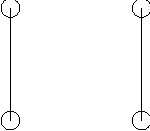
\includegraphics[scale = 0.75]{false-connect-cx}
\end{figure}
}

\item Since the Claim is false, there must be a logical mistake in the
following bogus proof.  Pinpoint the \emph{first} logical mistake
(unjustified step) in the proof.

\begin{proof}
  We prove the Claim above by induction.  Let $P(n)$ be the proposition
  that if every vertex in an $n$-vertex graph has positive degree, then
  the graph is connected.

\textbf{Base cases}: ($n \leq 2$).  In a graph with 1 vertex, that vertex
cannot have positive degree, so $P(1)$ holds vacuously.

$P(2)$ holds because there is only one graph with two vertices of positive
degree, namely, the graph with an edge between the vertices, and this
graph is connected.

\textbf{Inductive step}: We must show that $P(n)$ implies
$P(n+1)$ for all $n \geq 2$.  Consider an $n$-vertex graph in which every
vertex has positive degree.  By the assumption $P(n)$, this graph is
connected; that is, there is a path between every pair of vertices.  Now
we add one more vertex $x$ to obtain an $(n+1)$-vertex graph:

\mfigure{!}{1.75in}{false-connect-pic}

All that remains is to check that there is a path from $x$ to every other
vertex $z$.  Since $x$ has positive degree, there is an edge from $x$ to
some other vertex, $y$.  Thus, we can obtain a path from $x$ to $z$
by going from $x$ to $y$ and then following the path from $y$ to $z$.  This
proves $P(n+1)$.

By the principle of induction, $P(n)$ is true for all $n \geq 0$, which
proves the Claim.

\end{proof}

\solution{
This one is tricky: the proof is actually a good proof of
something else.  The first error in the proof is only in the final
statement of the inductive step: ``This proves $P(n+1)$''.

The issue is that to prove $P(n+1)$, \emph{every} $(n+1)$-vertex
positive-degree graph must be shown to be connected.  But the proof
doesn't show this.  Instead, it shows that every $(n+1)$-vertex
positive-degree graph \emph{that can be built up by adding a vertex of
positive degree to an $n$-vertex connected graph}, is connected.

The problem is that \emph{not every} $(n+1)$-vertex positive-degree graph
can be built up in this way.  The counterexample above illustrates this:
there is no way to build that 4-vertex positive-degree graph from a
3-vertex positive-degree graph.

More generally, this is an example of ``buildup error''.  This error
arises from a faulty assumption that every size $n+1$ graph with some
property can be ``built up'' in some particular way from a size $n$ graph
with the same property.  (This assumption is correct for some properties,
but incorrect for others--- such as the one in the argument above.)

One way to avoid an accidental build-up error is to use a ``shrink
down, grow back'' process in the inductive step: start with a size
$n+1$ graph, remove a vertex (or edge), apply the inductive hypothesis
$P(n)$ to the smaller graph, and then add back the vertex (or edge)
and argue that $P(n+1)$ holds.  Let's see what would have happened if
we'd tried to prove the claim above by this method:

\noindent \textit{Inductive step:} We must show that $P(n)$ implies
$P(n+1)$ for all $n \geq 1$.  Consider an $(n+1)$-vertex graph $G$ in
which every vertex has degree at least 1.  Remove an arbitrary vertex
$v$, leaving an $n$-vertex graph $G'$ in which every vertex has
degree... uh-oh!

The reduced graph $G'$ might contain a vertex of degree 0, making the
inductive hypothesis $P(n)$ inapplicable!  We are stuck--- and
properly so, since the claim is false!
}

\end{enumerate}

\section{The Grow Algorithm}

Yesterday in lecture, we saw the following algorithm for constructing
a minimum-weight spanning tree (MST) from an edge-weighted $N$-vertex 
graph $G$.\\

ALG-GROW:
\begin{enumerate}
\item Label the edges of the graph $e_1, e_2, \ldots , e_t$ so that
  $wt(e_1)\leq wt(e_2) \ldots \leq wt(e_t)$.
\item Let $S$ be the empty set.
\item For $i=1\ldots t$, if $S\cup \{e_i\}$ does not contain a cycle,
  then extend $S$ with the edge $e_i$.
\item Output $S$.
\end{enumerate}

\insolutions{

In summary, ALG-GROW selects edges one at a time, always choosing the
minimum weight edge that does not create a cycle with previously
selected edges. Notice that as edges are added $S$ may not be 
connected. When the algorithm terminates, $S$ contains $N-1$ edges. If
it is connected, then it is a spanning tree.

Consider, for example, the following edge-weighted graph.

\mfigure{!}{1.75in}{weightedGraph}

Now suppose we run ALG-GROW on our graph. We may choose the weight $1$
edge on the bottom of the triangle of weight $1$ edges in our
graph. In the next step, we may choose the weight $1$ edge on the top
of the graph. Note that this edge still has minimum weight, and does
not cause us to form a cycle, so ALG-GROW can choose it. We will then
choose one of the remaining weight $1$ edges. Note that neither causes
us to form a cycle. Continuing the algorithm, we may end up with the
same spanning tree shown below.

\mfigure{!}{2in}{exampleAlg}

In this recitation, we will analyze ALG-GROW.

}

\subsection{Analysis of ALG-GROW}

In this problem you may assume the following lemma from 
the problem set:
\begin{lemma}\label{n1}
Suppose that $T = (V, E)$ is a simple, connected graph. Then $T$ is a
tree iff $|E| = |V|-1$.
\end{lemma}

\instatements{\vspace{.2in}}

In this exercise you will prove the following theorem.

\begin{theorem*}
For any connected, weighted graph $G$, ALG-GROW produces an MST of $G$. 
\end{theorem*}

\instatements{\vspace{.2in}}

\newcounter{Lcount}
\begin{list}{\textbf{(\alph{Lcount})}}
{\usecounter{Lcount}}

\item Prove the following lemma.
\begin{lemma}\label{cycle}
Let $T=(V,E)$ be a tree and let $e$ be an edge not in $E$. Then,
$G=(V,E\cup \{e\})$ contains a cycle.
\end{lemma}
(Hint: Suppose $G$ does \emph{not} contain a cycle. Is $G$ a tree?)

\solution{
\begin{proof}(by contradiction)
Suppose $G$ does not contain a cycle. By the definition of a tree, $T$
is connected. Notice that $T$ is a subgraph of $G$. Because any two
nodes in $G$ are connected by a path in $T$, $G$ is a connected graph.
So $G$ is connected and acyclic and therefore a tree by
definition. Both $G$ and $T$ are trees and have the same number of
nodes. Therefore, they have the same number of edges (by
Lemma~\ref{n1}). This is a contradiction because $G$ has one more
edge than $T$.
\end{proof}
}

\item
Prove the following lemma.

\begin{lemma} \label{edge}
Let $T=(V,E)$ be a spanning tree of $G$ and let $e$ be an edge 
not in $E$. Then there exists an edge $e'\neq e$ in $E$ such that
$T^*=(V,E-\{e'\} \cup \{e\})$ is a spanning tree of $G$.
\end{lemma}
(Hint: Adding $e$ to $E$ introduces a cycle in $(V,E\cup\{e\})$.)

\solution{
\begin{proof}
By Lemma~\ref{cycle}, we know that the set of edges $E\cup \{e\}$
contains a cycle. If this cycle does not contain the edge $e$, then
this cycle is a subset of $E$. Since $E$ is the set of edges of a
tree, this cannot occur. So, this cycle contains $e$. If $e'$ is
another edge distinct from $e$ in this cycle, then the graph $T^*$
that results after removing $e'$ from $E\cup \{e\}$ is still
connected. The number of edges in $T^*$ is equal to the number of
edges in $T$, which is equal to $|V|-1$ by Lemma~\ref{n1}. Since
$T^*$ is connected, $T^*$ is a tree by Lemma~\ref{n1}. Since $T^*$ is
a subgraph of $G$ with vertices $V$, it spans $G$.
\end{proof}
}

\item
Prove the following lemma.

\begin{lemma} \label{edge2}
Let $T=(V,E)$ be a spanning tree of $G$, let $e$ be an edge not in
$E$ and let $S\subseteq E$ such that $S\cup \{e\}$ does not contain a
cycle.  Then there exists an edge $e'\neq e$ in $E-S$ such that
$T^*=(V,E-\{e'\} \cup \{e\})$ is a spanning tree of $G$.
\end{lemma}
(Hint: Modify your proof to part (b). Of all possible edges $e'\neq e$ that can be removed to construct $T^*$, at least one is not in $S$.)

\solution{
\begin{proof}
We need to change the proof in part (b) slightly. The proof of part (b)
holds for any edge $e'\neq e$ in the cycle. We need to show that we can
select an edge $e'\neq e$ that is in the cycle but not in $S$. We will
prove this by contradiction. Suppose that all the edges not equal to
$e$ that are in the cycle are in $S$. Then, $S\cup e$ is a cycle. This
contradicts the assumption of the lemma.
\end{proof}
}

\item
Prove the following lemma.

\begin{lemma} \label{magic}
Define $S_m$ to be the set consisting of the first $m$ edges selected by 
ALG-GROW from a connected graph $G$. Let $P(m)$ be the predicate that if 
$m \leq |V|$ then $S_m \subseteq E$ for some MST $T=(V,E)$ of $G$. Then
$\forall m \; . \; P(m).$
\end{lemma}
(Hint: Use induction. There are two cases: $m+1 > |V|$ and $m+1 \leq |V|$. In the second case, there are two subcases.)

\solution{
\begin{proof}(By induction.)
Let $P(m)$ be the predicate as defined above.

Base Case: $S_0$ contains 0 edges and is equal to the empty set,
which is a subset of any set of edges $E$.

Inductive Step: Assume $P(m)$ in order to prove $P(m+1)$.

If $m \geq |V|$ then $m+1 > |V|$ and $P(m+1)$ holds 
vacuously.  Otherwise, if $m < |V|$ then let $e$ denote
the $(m+1)$th edge selected by ALG-GROW. By the inductive hypothesis,
there exists an MST $T = (V, E)$ such that $S_m \subseteq E$. There are
now two cases.

In the first case, $e \in E$ which case $S_m \cup \{e\} \subseteq E$,
and thus $P(m+1)$ holds.

In the second case, $e \notin E$, as illustrated by the following
diagram. Now we need to find a different MST that contains 
$S_m \cup \{e\}$.

\mfigure{!}{2in}{MSTproof}

What happens when we add $e$ to $T$? By the description of ALG-GROW,
$S_m \cup \{e\}$ does not contain a cycle. Therefore, by Lemma~\ref{edge2},
there exists an edge $e'\neq e$ in $E-S_m$ such that
$T^*=(V,E-\{e'\} \cup \{e\})$ is a spanning tree for $G$.

In order to prove that $T^*$ is a MST, we need to show that
$wt(e)\leq wt(e')$. We will prove this by contradiction. Suppose that
$wt(e')< wt(e)$. Since $e'\in E$, which is the set of edges of the MST
$T$, and $S_m \subseteq E$, the set of edges $S_m \cup \{e'\}$, does not
contain a cycle. Therefore $e'$ would have already been added to $S_m$
in a previous iteration of ALG-GROW as one of the first $m$
edges. However, $e'$ is in $E-S_m$. This is a contradiction.
\end{proof}
}

\item
Prove the theorem. (Hint: Lemma~\ref{magic} says there exists an MST $T=(V,E)$ for $G$ such that $S\subseteq E$. Use contradiction to rule out the case in which $S$ is a proper subset of $E$.)

\solution{
\begin{proof}(by contradiction)
Let $S$ be the set of edges produced by ALG-GROW. By
Lemma~\ref{magic}, there exists an MST $T=(V,E)$ for $G$ such that
$S\subseteq E$. If $S=E$, then ALG-GROW outputs the edges of the MST
$T$. 

We will show that the other case, $S\neq E$, leads to a
contradiction. Suppose $S\neq E$. Then there exists an edge $e\in
E-S$. This implies that $S\cup \{e\}\subseteq E$. Since $E$ is the set
of edges of a tree, $S\cup \{e\}$ does not contain a cycle. Therefore,
$e$ would be added to $S$ by ALG-GROW. So $e\in S$, and this
contradicts $e\in E-S$.

\end{proof}
}

\end{list}

\end{document}
